\documentclass[crop,tikz]{standalone}
\usepackage{pgfplots}
\pgfplotsset{compat=1.13}

% Lines of constant potential for an upper half of a cylinder of
% radius 1 at position (x,y) = (0,0).
%
% Inspired by the discussion in
% https://galileoandeinstein.phys.virginia.edu/Elec_Mag/2022_Lectures/EM_16_Conformal_Mapping.html

\pgfplotsset{
  inverted/.style = {
    every axis legend/.append style={
      draw=white,
      fill=hardblack,
      text=white
    }
  },
  every non boxed x axis/.append style={
    axis line style={-latex}
  },
  every non boxed y axis/.append style={
    axis line style={-latex}
  }
}

\begin{document}

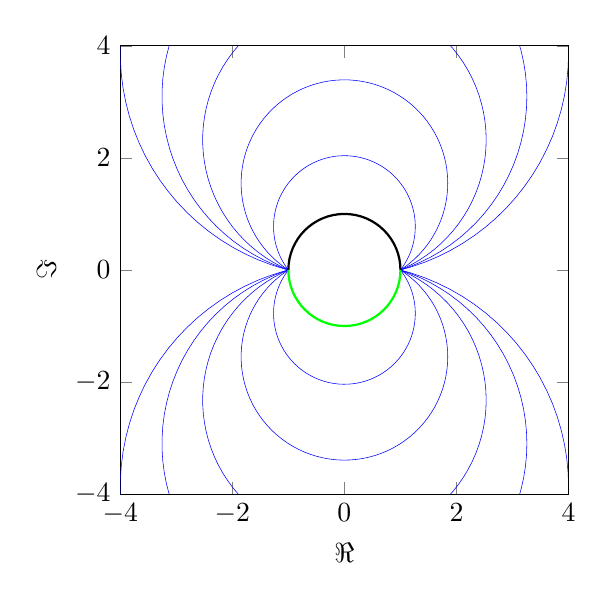
\begin{tikzpicture}
  \pgfmathsetmacro{\numberofpotentiallines}{10};
  \pgfmathsetmacro{\rmin}{1.1}; % minimum radius outside
  \pgfmathsetmacro{\rmax}{4}; % maximum radius outside
  \pgfmathsetmacro{\remin}{-4};
  \pgfmathsetmacro{\remax}{-\remin};
  \pgfmathsetmacro{\immin}{-4};
  \pgfmathsetmacro{\immax}{-\immin};
  \begin{axis}[
    axis equal image,
    xmin={\remin}, xmax={\remax},
    ymin={\immin}, ymax={\immax},
    xlabel={$\Re$},
    ylabel={$\Im$},
    samples=100,
    domain=0:360,
    declare function = {
      % lines of constant potential
      phir(\c) = sqrt(1 + \c^2); % radius
      phix(\x,\c) = phir(\c)*cos(\x); % x coordinate
      phiy(\x,\c) = phir(\c)*sin(\x) + \c; % y coordinate
      fc(\n,\nmax) = (\n/\nmax*2 - 1)*sqrt(\rmax^2 - 1); % calculates c
    },
    ]
    \begin{scope}[even odd rule]
      \clip ({\remin},{\immin}) rectangle ({\remax},{\immax}) (0,0) circle (1);
      % lines of constant potential outside
      \pgfplotsinvokeforeach{0,...,{\numberofpotentiallines}}{
        \addplot[blue,very thin] (
        {phix(x, fc(#1,\numberofpotentiallines))},
        {phiy(x, fc(#1,\numberofpotentiallines))}
        );
      }
    \end{scope}
    % upper half (potential V1 != 0)
    \draw[thick] (1,0) arc (0:180:1);
    % lower half (potential V2 = 0)
    \draw[thick,green] (-1,0) arc (180:360:1);
  \end{axis}
\end{tikzpicture}
\end{document}
